\subsection{Hardware}
The smart wheelchair must sense the environment, process this information,
and maneuver within the environment. Doing so requires hardware, including a
sensor system, compute unit, and motor controller.

The literature review compares several types of sensors and manufacturers for these sensors.
An RGB-D camera was selected for this application, as they provide high-resolution images and depth
information at a commercially viable price point. High-resolution image data builds flexibility into
the system, as popular machine learning algorithms can be utilised.

This RGB-D camera must be mounted to the wheelchair at an appropriate point. The front of the
joystick control unit was selected for the reasons below:
\begin{enumerate}[topsep=0pt,itemsep=-1ex,partopsep=1ex,parsep=1ex]
    \item A clear view of the environment in front of the wheelchair is provided.
    \item The user does not obstruct the camera's view in any wheelchair configuration.
    \item The camera does not obstruct the user's view or comfort in any wheelchair configuration.
    \item When exiting the wheelchair, the user can move the joystick control unit and camera
            out of the way using the existing joystick control unit mount.
\end{enumerate}
Some considerations must be addressed when using this mounting point.
\begin{enumerate}[topsep=0pt,itemsep=-1ex,partopsep=1ex,parsep=1ex]
    \item Unstable video footage could be observed due to low rigidity in the joystick control unit mount.
    \item Mount point is \SI{790}{\milli\metre} forward from the back of the wheelchair, impacting
            the visibility of the rear and side of the wheelchair.
    \item Doorway maneuverability is impacted if RGB-D camera width exceeds \SI{150}{\milli\metre}.
\end{enumerate}
This sensor mounting point is positioned on the right-hand side of the wheelchair,
\SI{720}{\milli\metre} above the ground and \SI{300}{\milli\metre} behind the
front of the wheelchair (measured from the footplate), and can be seen in \cref{fig:wheelchair_zed_1}.

The RGB-D camera model selected was the Stereolabs ZED Mini, which uses passive stereo-vision
to generate a depth map. Active IR RGB-D cameras were not viable for this application
due to their poor outdoor performance and range. The width of the ZED Mini also fulfils the
size requirements of the selected mounting point.

Smart wheelchair applications such as wheelchair docking require
obstacle detection on all sides of the wheelchair. To satisfy this requirement, a
Cygbot CygLiDAR D1 was procured for short-range detection of obstacles at the rear of the
wheelchair. Nicolas Lee, a project student focused on
wheelchair navigation to personal vehicles, selected this sensor. It should be noted that
this sensor was not used for navigation assistance as part of this thesis.

% Sensor mount design
A 3D printed sensor mount was designed to fix the ZED Mini to the wheelchair mounting point.
This sensor mount was based on a ZED Mini mount designed by Walter Lucetti at Stereolabs \cite{lucettiStereolabsZEDMini2018},
with several major modifications made using Autodesk Inventor:
\begin{enumerate}[topsep=0pt,itemsep=-1ex,partopsep=1ex,parsep=1ex]
    \item Width of the mount was greatly reduced to improve maneuverability.
    \item A mounting plate was added, allowing the sensor mount to bolt onto
            the existing joystick control unit.
    \item Some sensor clips were modified to make sensor removal more convenient.
    \item Sharp corners were rounded to reduce the risk of injury to a user.
\end{enumerate}
\Cref{fig:zed_mount} shows a render of the ZED Mini camera and custom mount.
\Cref{fig:wheelchair_zed_1} shows the ZED Mini camera mounted to the joystick control unit
on the wheelchair.

\begin{figure}[b]
    \centering
    \begin{minipage}[b]{.4\textwidth}
      \centering
      \captionsetup{width=.8\textwidth}
      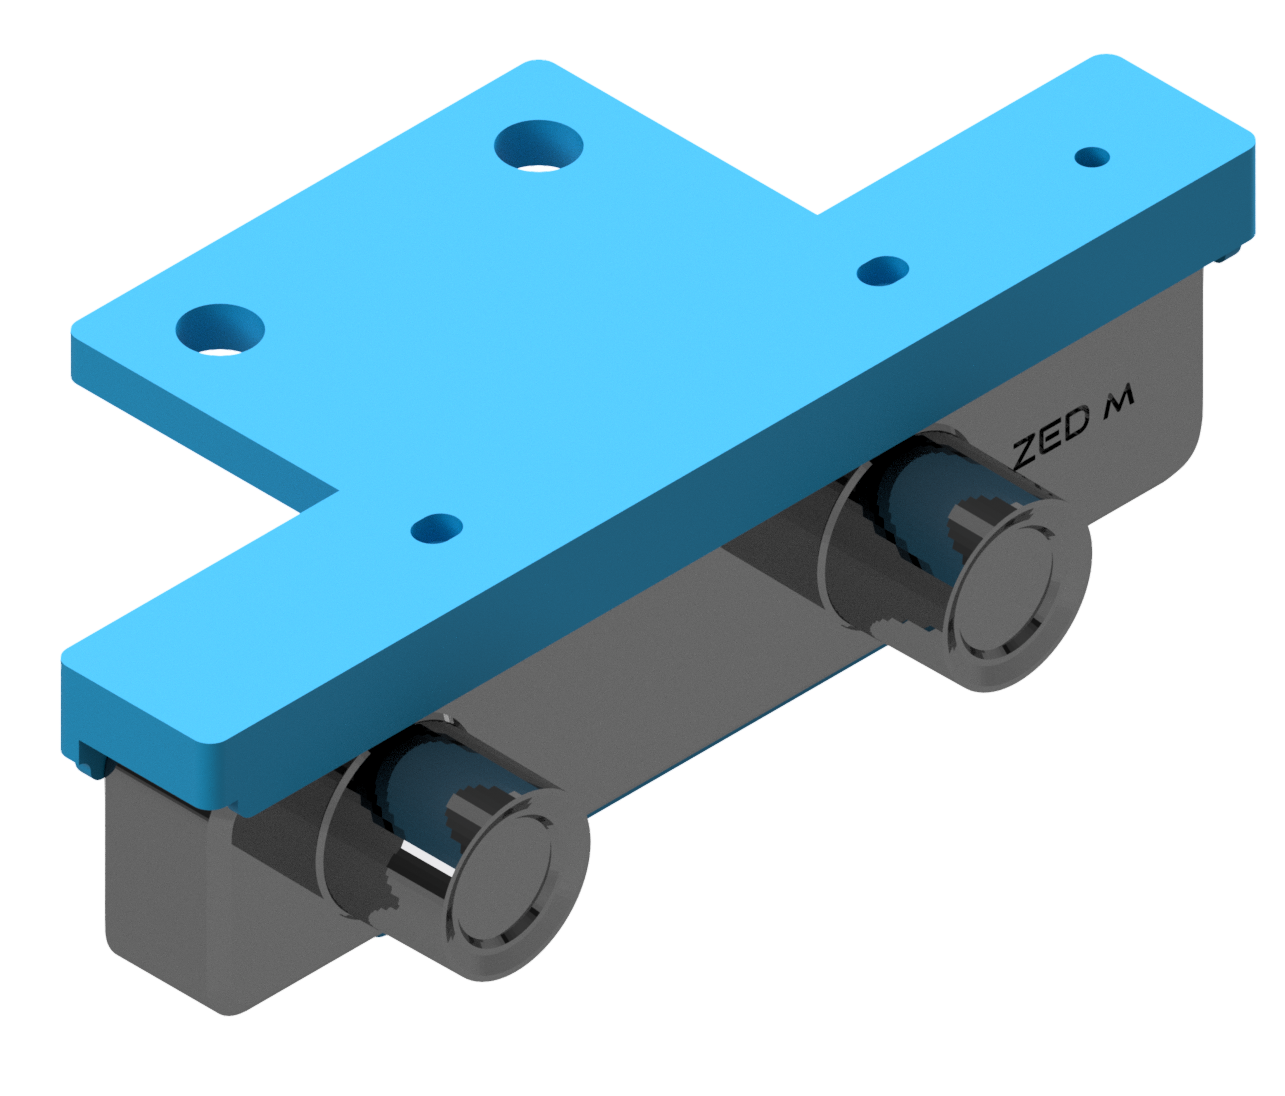
\includegraphics[width=\linewidth]{images/zed_mount.png}
        \captionof{figure}{3D render of ZED Mini camera and wheelchair mount}
        \label{fig:zed_mount}
    \end{minipage}%
    \begin{minipage}[b]{.48\textwidth}
        \centering
        \captionsetup{width=.8\textwidth}
        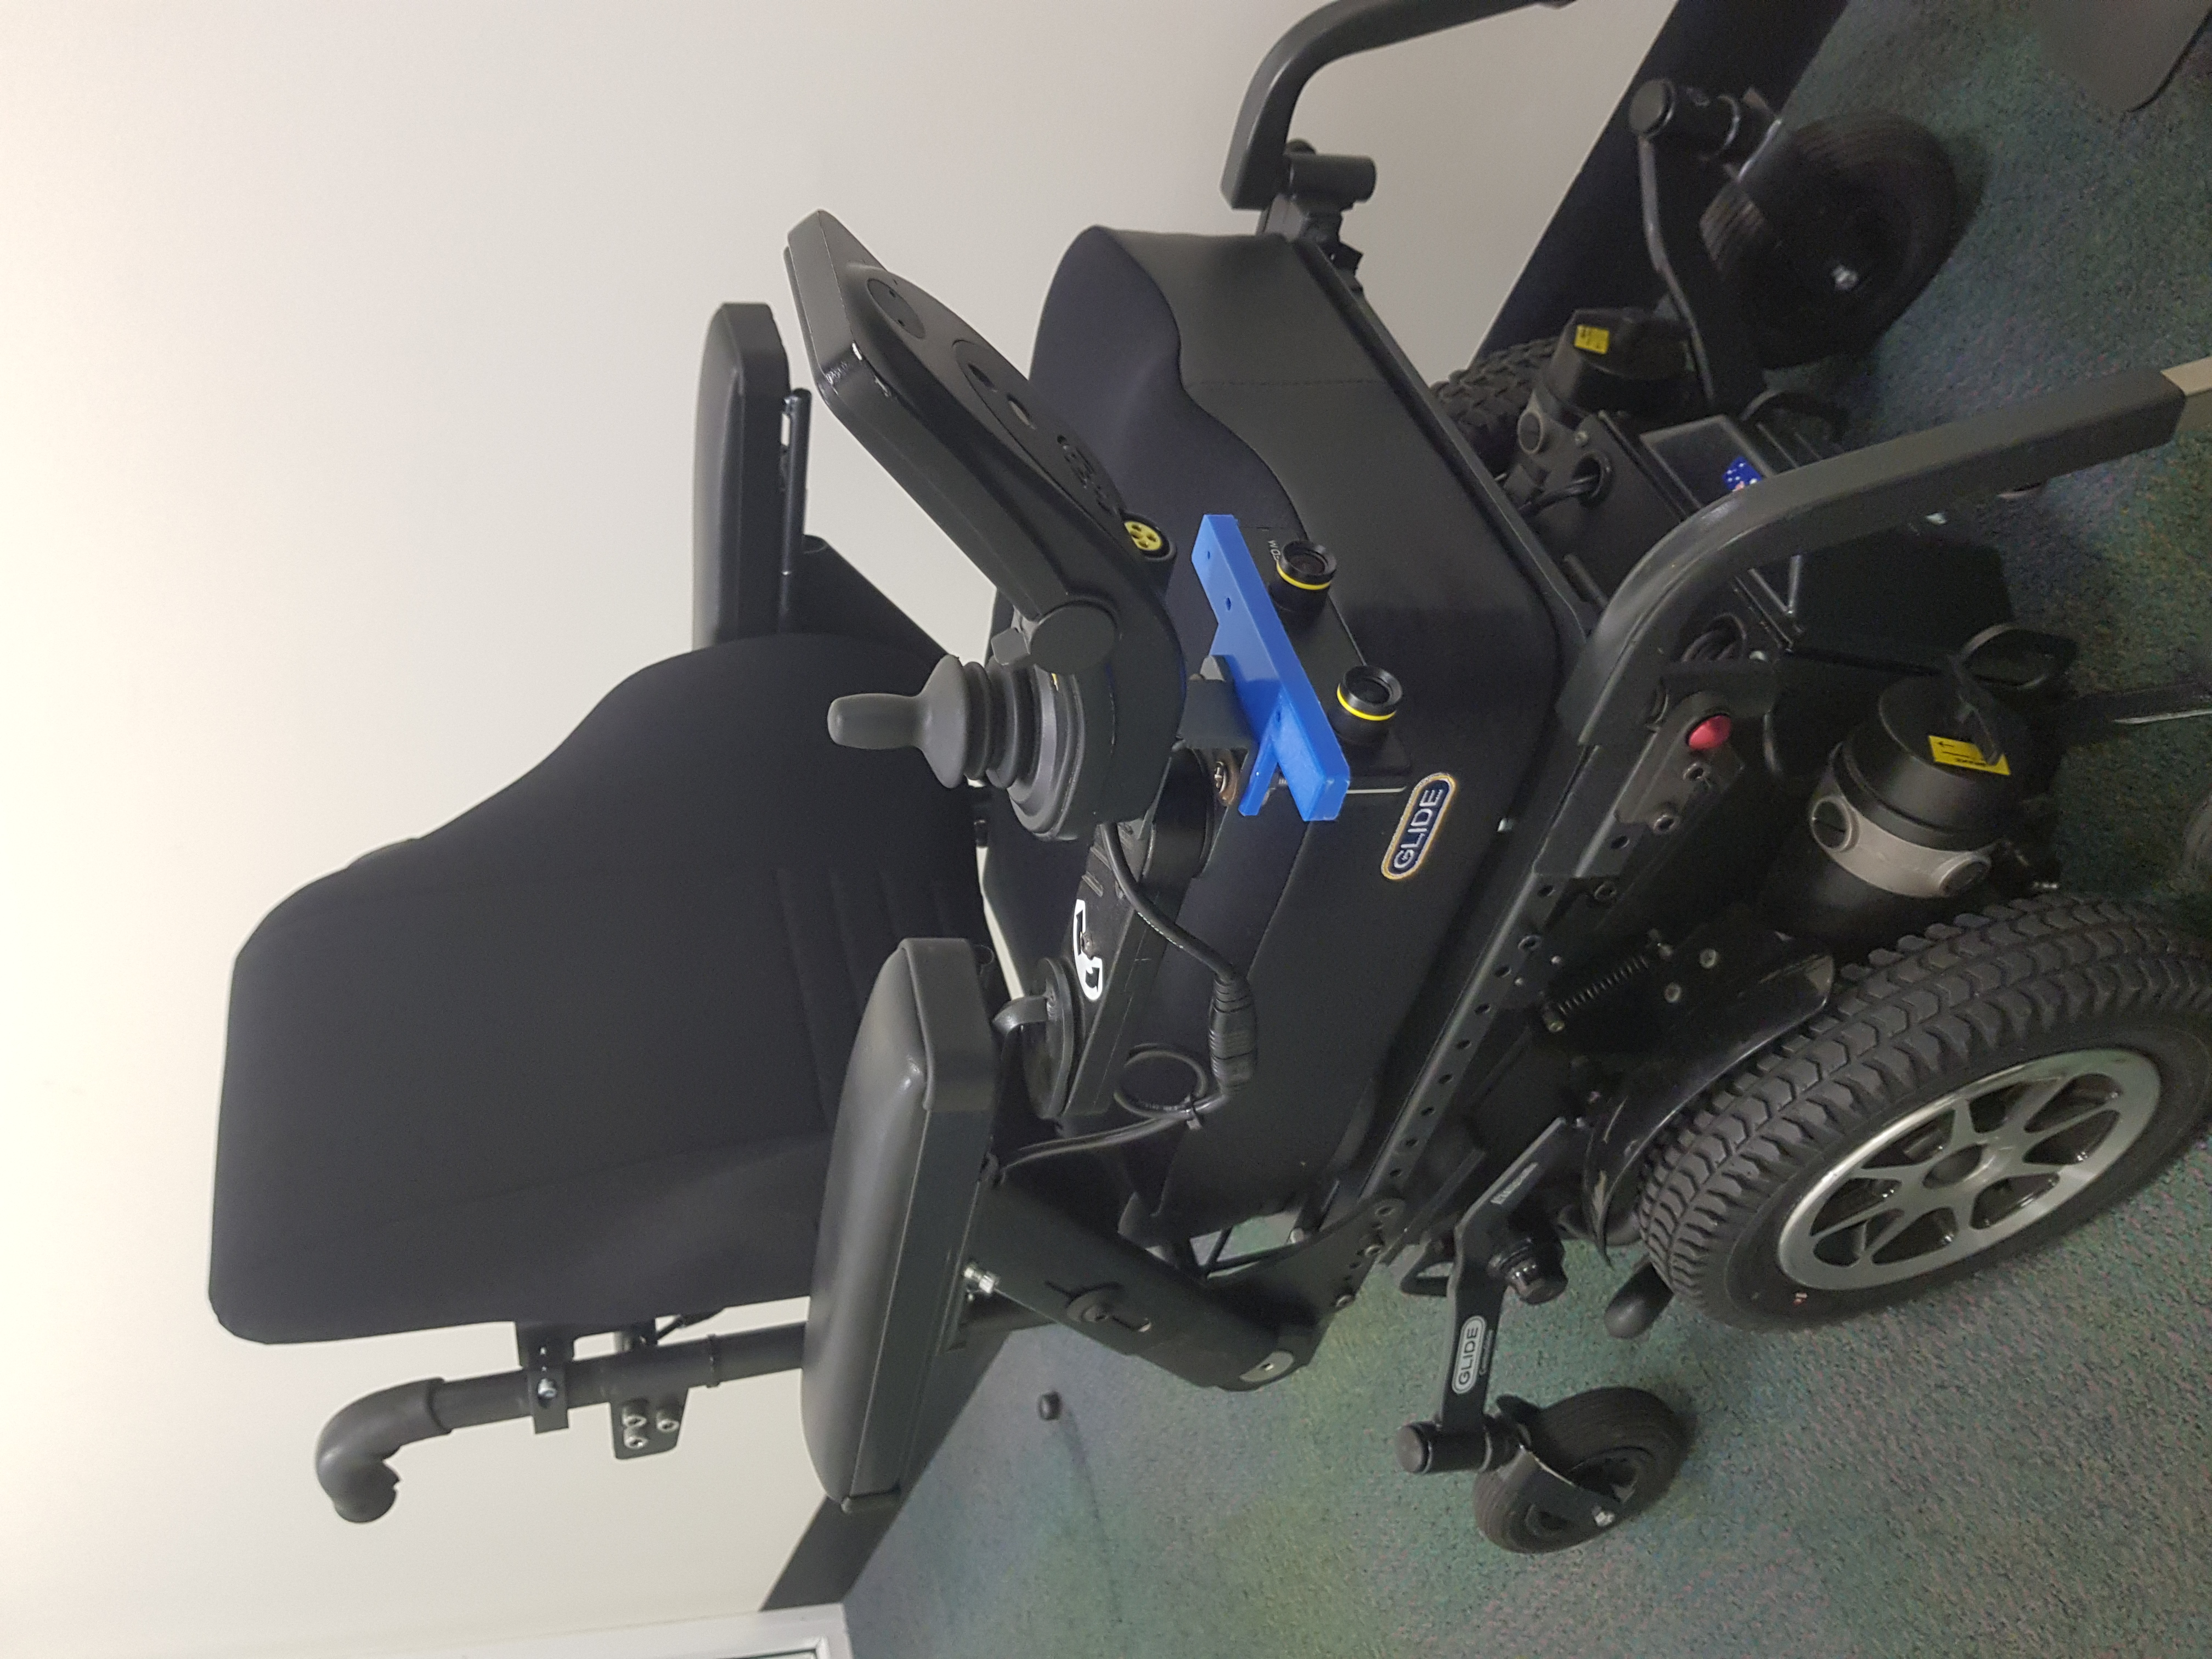
\includegraphics[height=\linewidth,angle=270,origin=c]{images/wheelchair_zed_1.jpg}
        \captionof{figure}{ZED Mini camera and mount fixed to joystick control unit}
        \label{fig:wheelchair_zed_1}
    \end{minipage}
\end{figure}

In addition to the RGB-D camera and Lidar sensor, an AI accelerator is required to process the sensors'
output and run ML algorithms. The literature review compares several AI accelerators across categories
such as computational speed, power draw, and price. An Nvidia Jetson Xavier NX was selected for this task,
as the Stereolabs ZED Mini requires a CUDA-enabled accelerator to generate a depth map. This accelerator's
low power draw and small form factor are suited for mobile robot applications such as smart wheelchairs.
Due to budget constraints and the ongoing chip shortage, the project team could not procure this AI accelerator.
Instead, a laptop with an RTX 3080 graphics card was used to record datasets and evaluate the speed of
ML algorithms.

A CentroGlide powered wheelchair was used as a base for the smart wheelchair functionality.
The CentroGlide is a mid-wheel drive wheelchair with two independently controlled powered wheels and four
unpowered castor wheels.
A joystick module communicates user commands to a power module, which controls
each motor. An intelligent seating module (ISM) adjusts the seat tilt and recline \cite{glideCentroGlideOWNERUSER2022}.
This wheelchair is \SI{1100}{\milli\metre} in length (including footplate), \SI{620}{\milli\metre}
in width, and \SI{1030}{\milli\metre} in height.
Communication between the joystick module, power module, and ISM is shown in \cref{fig:module_communication}.

\begin{figure}[b]
    \centering
    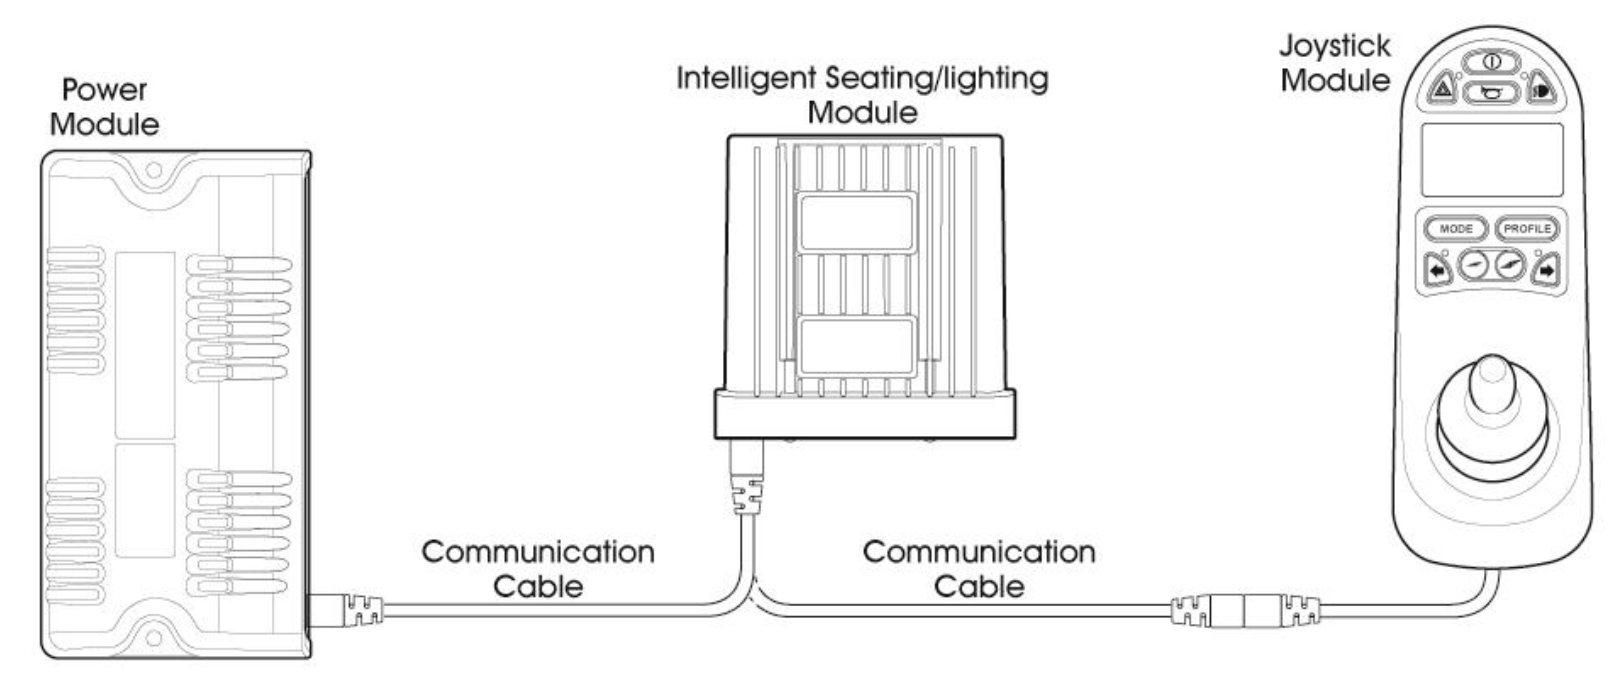
\includegraphics[width=0.85\linewidth]{images/module_communication.png}
    \caption{Communication between CentroGlide control modules. Reproduced from Curtiss-Wright. \cite{curtiss-wrightPGDRIVESTECHNOLOGY2016}}
    \label{fig:module_communication}
\end{figure}

An input controller is being developed by project student Brian Smith to intercept
commands from the joystick module and communicate with the smart wheelchair navigation system.
The input controller enables the navigation system to receive user commands and choose a safe
direction and speed for the wheelchair.
%A high-level protocol between the navigation system and input controller has been designed
%and is detailed in the future work section of this thesis.
The input controller will validate the
navigation system's output, ensuring that the user
can still safely maneuver the wheelchair in the case of a software failure.
Additionally, a motor controller was developed by project student
Kosma Egan, which receives commands from the input controller to drive and monitor the motors.
\pagebreak

\subsection{Data Collection}
\label{sec:dataset_collection}

An RGB-D wheelchair driving dataset was collected around Curtin university
to test and evaluate the performance of the navigation assistance system.
This dataset is \SI{7.14}{\giga\byte} in size and \SI{47}{\minute} in length
and includes features such as indoor and outdoor navigation, doorways, pedestrians,
elevator use, wheelchair access ramps, and car parks. A link to the dataset
can be found in Appendix B.

This dataset was collected using the ZED Mini and is encoded in the proprietary Stereolabs SVO file format, which can be read using the ZED SDK.
This format includes image data from left and right cameras, IMU data, and metadata such as
timestamps. Depth map and point cloud data are not stored in the dataset and are instead generated when
the file is read using the ZED SDK. Image data was recorded at 1080p, 30fps for the left and right cameras.

Four compression modes are available during data collection: Lossless (PNG), Lossy (JPG), H.264 (Video),
and H.265. Both video compression modes require a CUDA-enabled device during data collection.
A 10-second sample dataset was recorded for each compression mode to evaluate image quality and
file size (results in \cref{table:dataset_compression_modes}). Due to the smaller file size, H.264 compression was used when collecting the wheelchair driving dataset.
\Cref{fig:zed_sample_dataset} shows an example image frame and depth map from the dataset.

\begin{table}[H]
    \centering
    \begin{adjustbox}{width=0.7\textwidth}
    \begin{tabular}{c c c c}
    \toprule
    Compression mode & File size & Relative increase & Image quality \\
    \midrule
    Lossless (PNG) & \SI{1240}{\mega\byte} & 41 & Ok \\
    Lossy (JPG) & \SI{640}{\mega\byte} & 21 & Some interlacing \\
    H.264 & \SI{30}{\mega\byte} & 1 & OK \\
    H.265 & \SI{30}{\mega\byte} & 1 & Some frame tearing \\
    \bottomrule
    \end{tabular}
    \end{adjustbox}
    \caption{Comparison between dataset compression modes}
    \label{table:dataset_compression_modes}
\end{table}

\begin{figure}[H]
    \centering
    \begin{subfigure}{.48\textwidth}
        \centering
        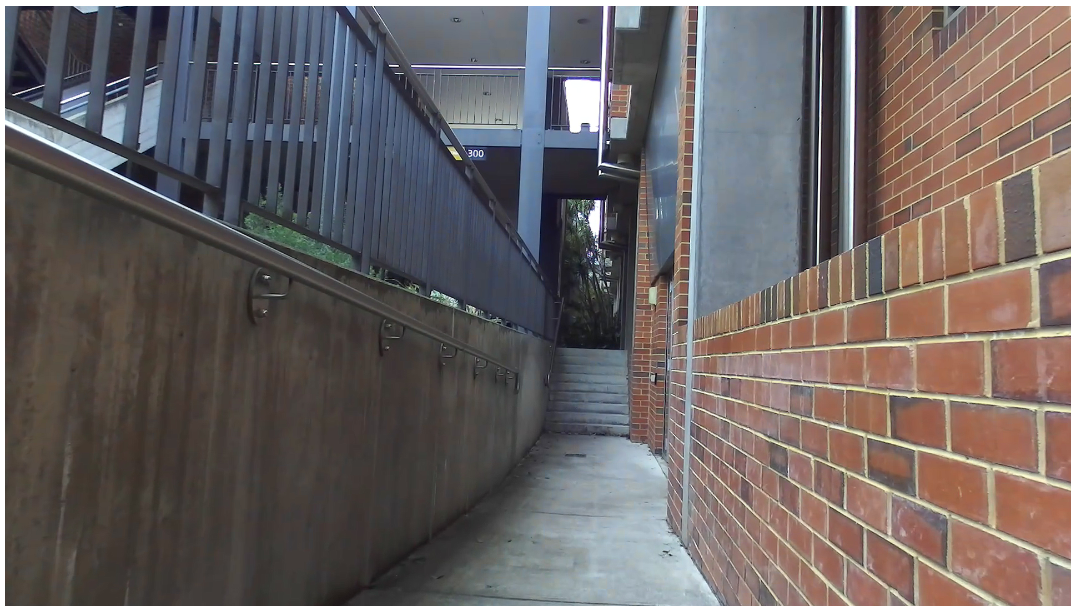
\includegraphics[width=\linewidth]{images/zed_sample_image.png}
        \caption{Image frame}
    \end{subfigure}
    \quad
    \begin{subfigure}{.47\textwidth}
        \centering
        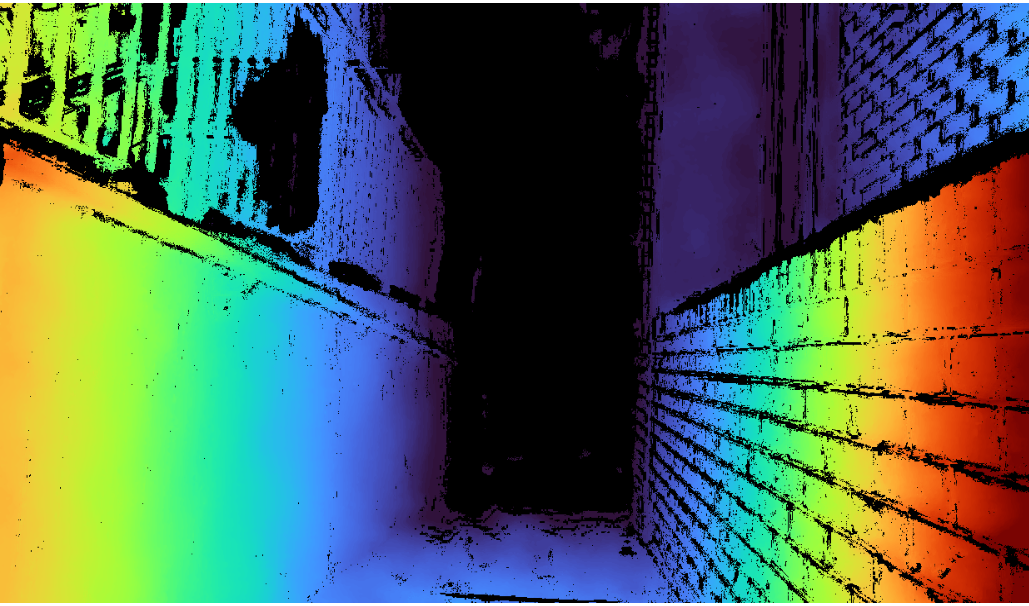
\includegraphics[width=\linewidth]{images/zed_sample_depth.png}
        \caption{Depth map}
    \end{subfigure}
    \caption{Sample data from the Curtin university RGB-D wheelchair driving dataset}
    \label{fig:zed_sample_dataset}
\end{figure}
\pagebreak

After some analysis of the raw point cloud data from the Curtin RGB-D driving dataset,
it was found that the camera was slightly tilted upwards while recording the dataset.
This angle was mostly constant between data collection periods
and was likely due to the ergonomics and tilt of the joystick control unit.
An example of this tilt can be seen in \cref{fig:meshlab_point_cloud}; note
that the floor is angled downwards due to the tilt of the RGB-D camera.

Meshlab was used to determine the coordinates of points
on the ground at a close distance and far distance, and calculate the gradient.
This was done for two different point clouds (one indoor and one outdoor)
with the results averaged. Working is shown in \cref{eq:tilt_calculation}.

\begin{equation}
\begin{split}
p_{1,1} = (-0.53, -1.30, -3.81) \qquad p_{1,2} &= (-0.54, -2.31, -11.31)\\
\textrm{gradient}_1 &= \frac{y_2 - y_1}{z_2 - z_1} = -0.135\\
p_{2,1} = (1.03, -1.29, -4.17) \qquad p_{2,2} &= (0.93, -2.80, -14.03)\\
\textrm{gradient}_2 &= -0.153\\
\textrm{gradient}_{avg} &= -0.144\\
\theta_{tilt} &= -\tan^{-1}\left(-0.144\right) = 8.2\degree
\end{split}
\label{eq:tilt_calculation}
\end{equation}

\begin{figure}[b]
    \centering
    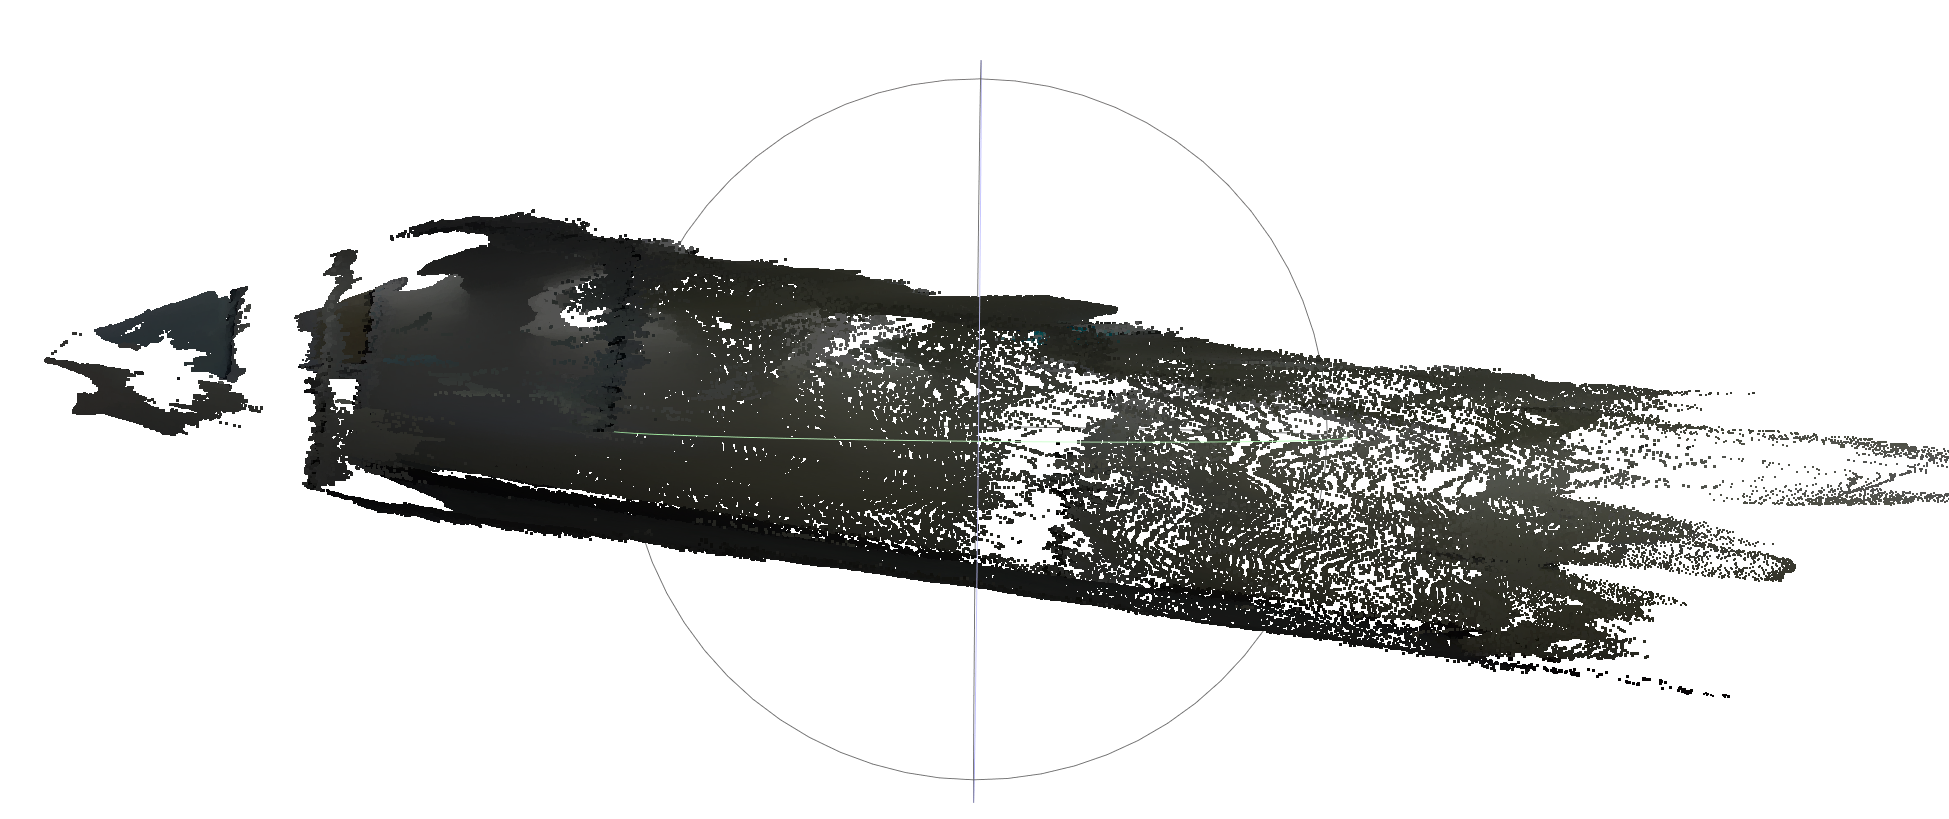
\includegraphics[width=0.8\linewidth]{images/meshlab_point_cloud.png}
    \caption{Point cloud information of indoor hallway (visualized with Meshlab). Note the angle of the floor due to sensor tilt}
    \label{fig:meshlab_point_cloud}
\end{figure}

In addition to the RGB-D dataset, a preliminary wheelchair driving video-only dataset was collected around
Curtin university.
This dataset was \SI{34}{\minute} in length and \SI{7.08}{\giga\byte} in size (1920x1080 @ 24 fps)
and collected using a GoPro Hero 4; the experimental setup used to collect this
dataset can be seen in \cref{fig:gopro_dataset_collection}.
This dataset was used to evaluate machine learning scene recognition algorithms
before the ZED Mini had been ordered.

%\vspace{4.0cm}
\begin{figure}[p]
    \centering
    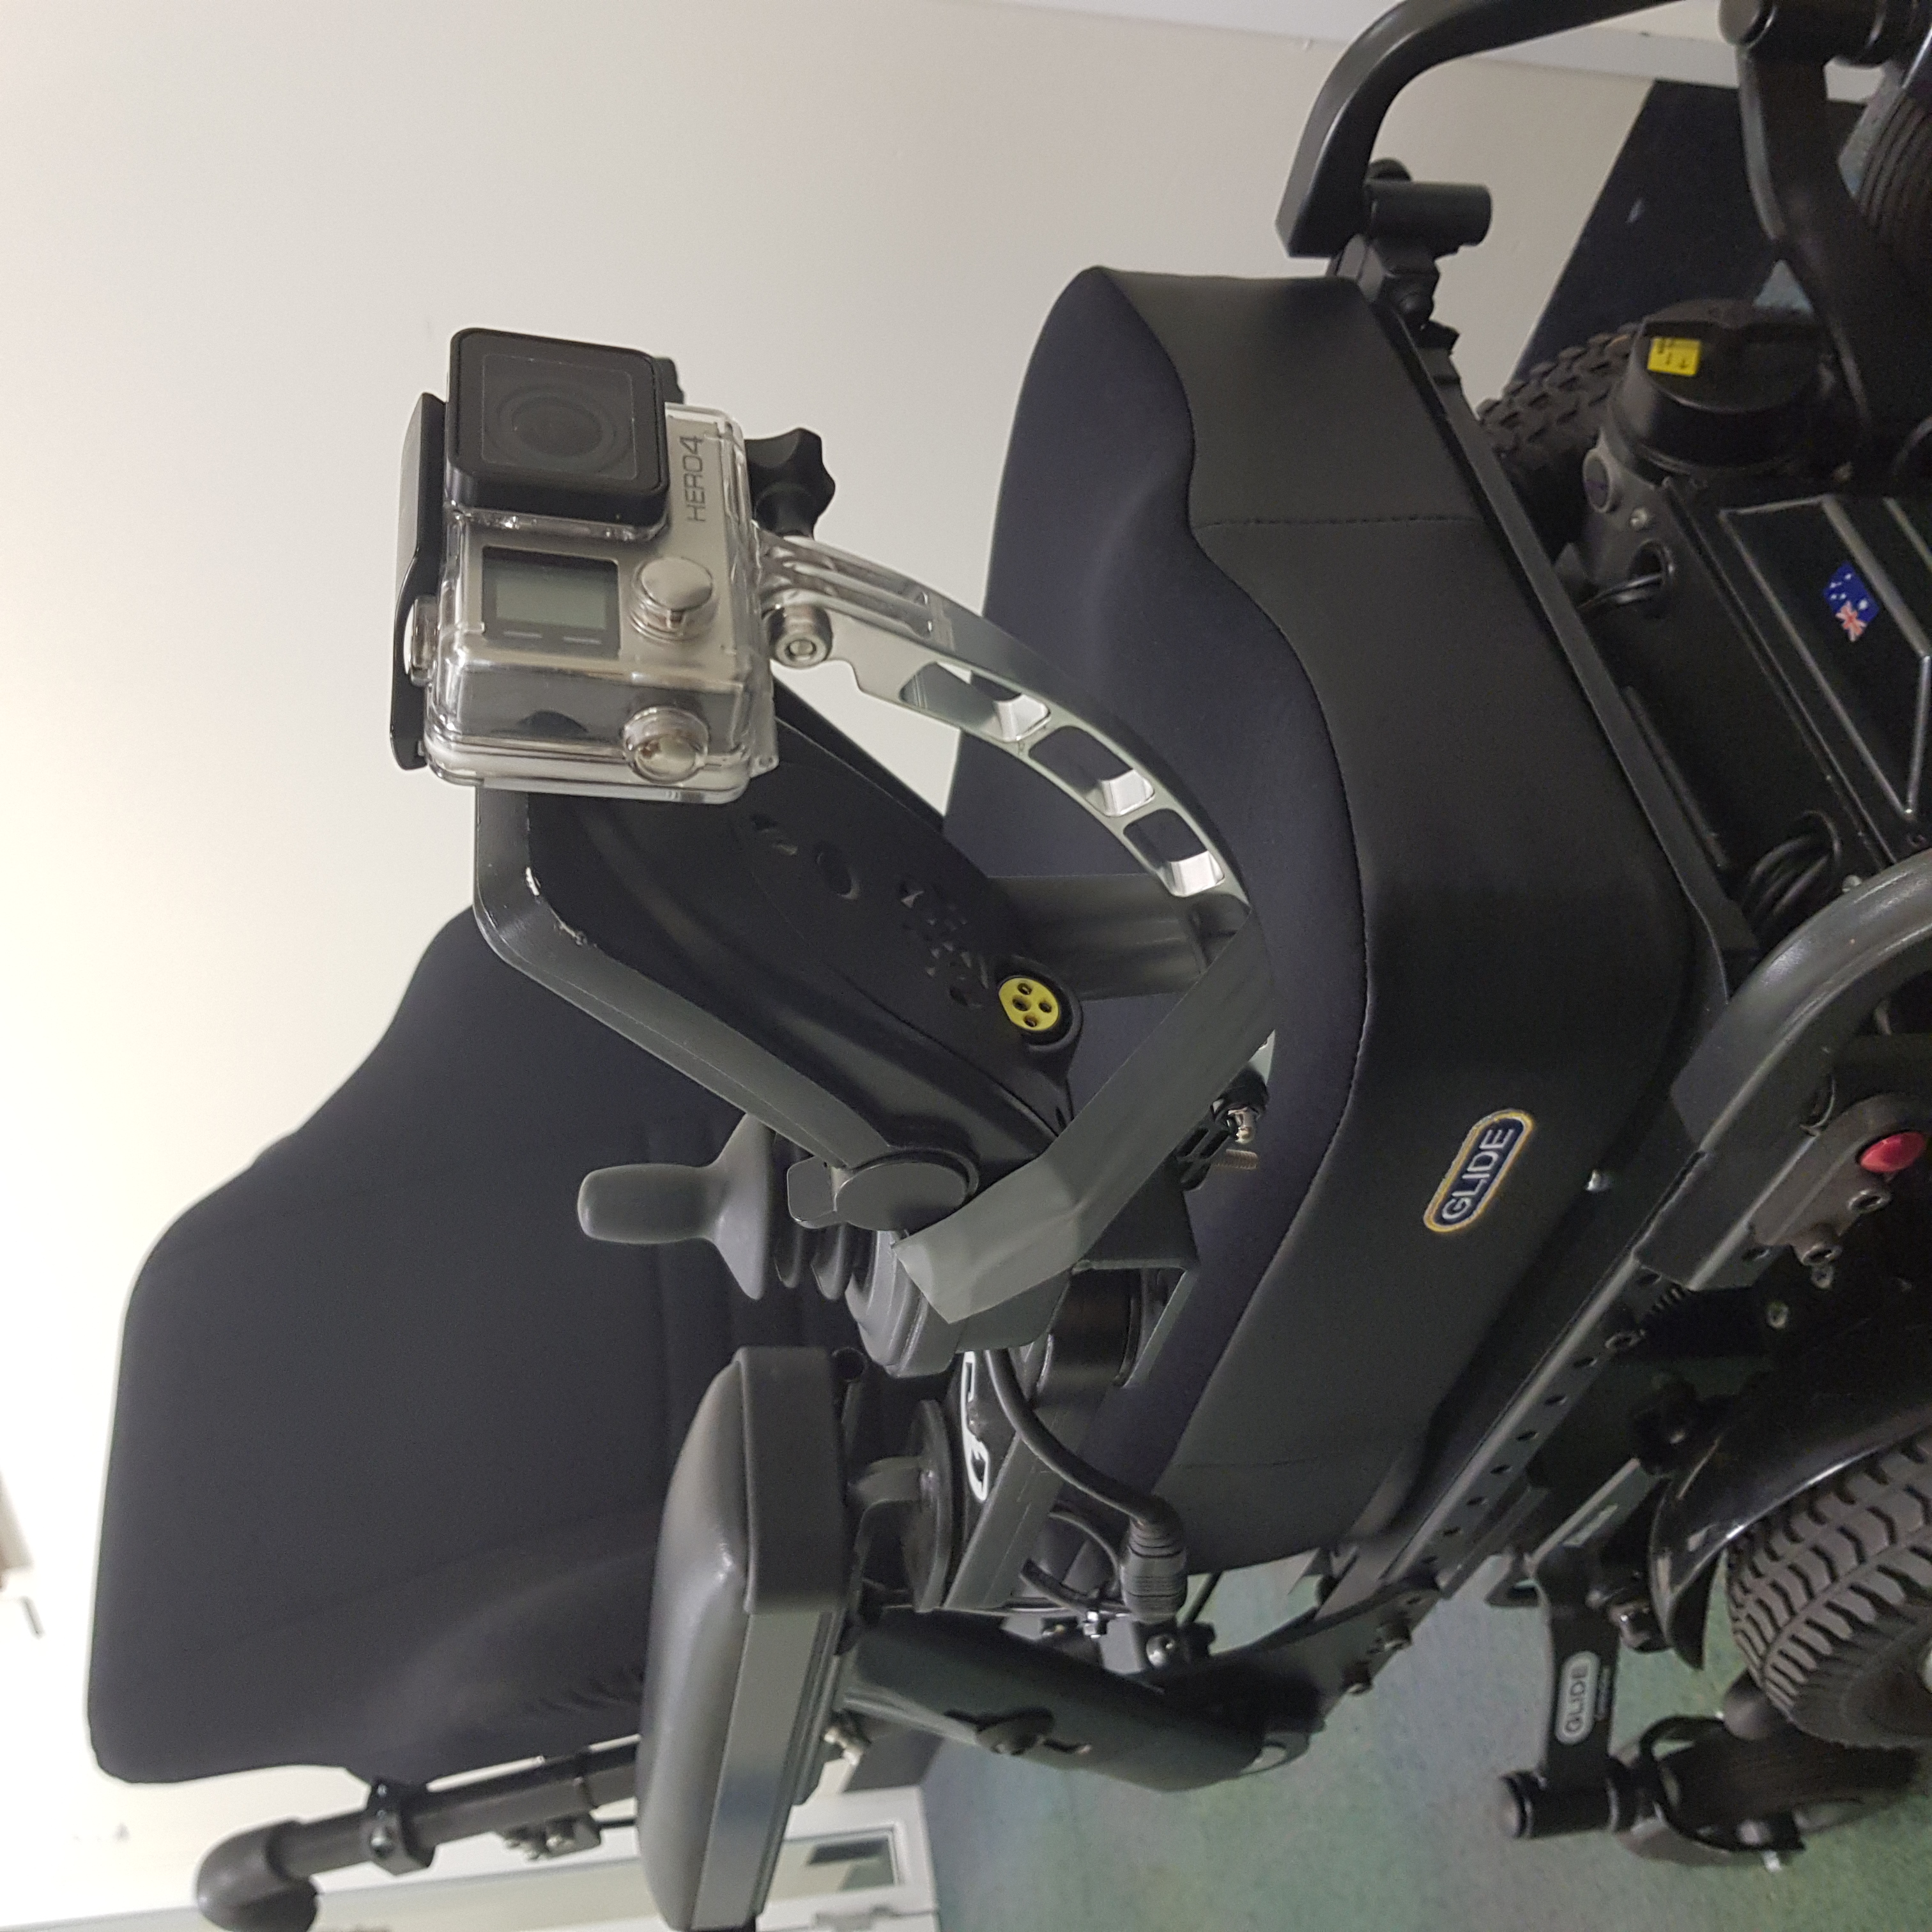
\includegraphics[width=0.45\linewidth,angle=270,origin=c]{images/gopro_dataset_collection.jpg}
    \caption{Experimental setup for preliminary data collection}
    \label{fig:gopro_dataset_collection}
\end{figure}

\begin{figure}[p]
    \centering
    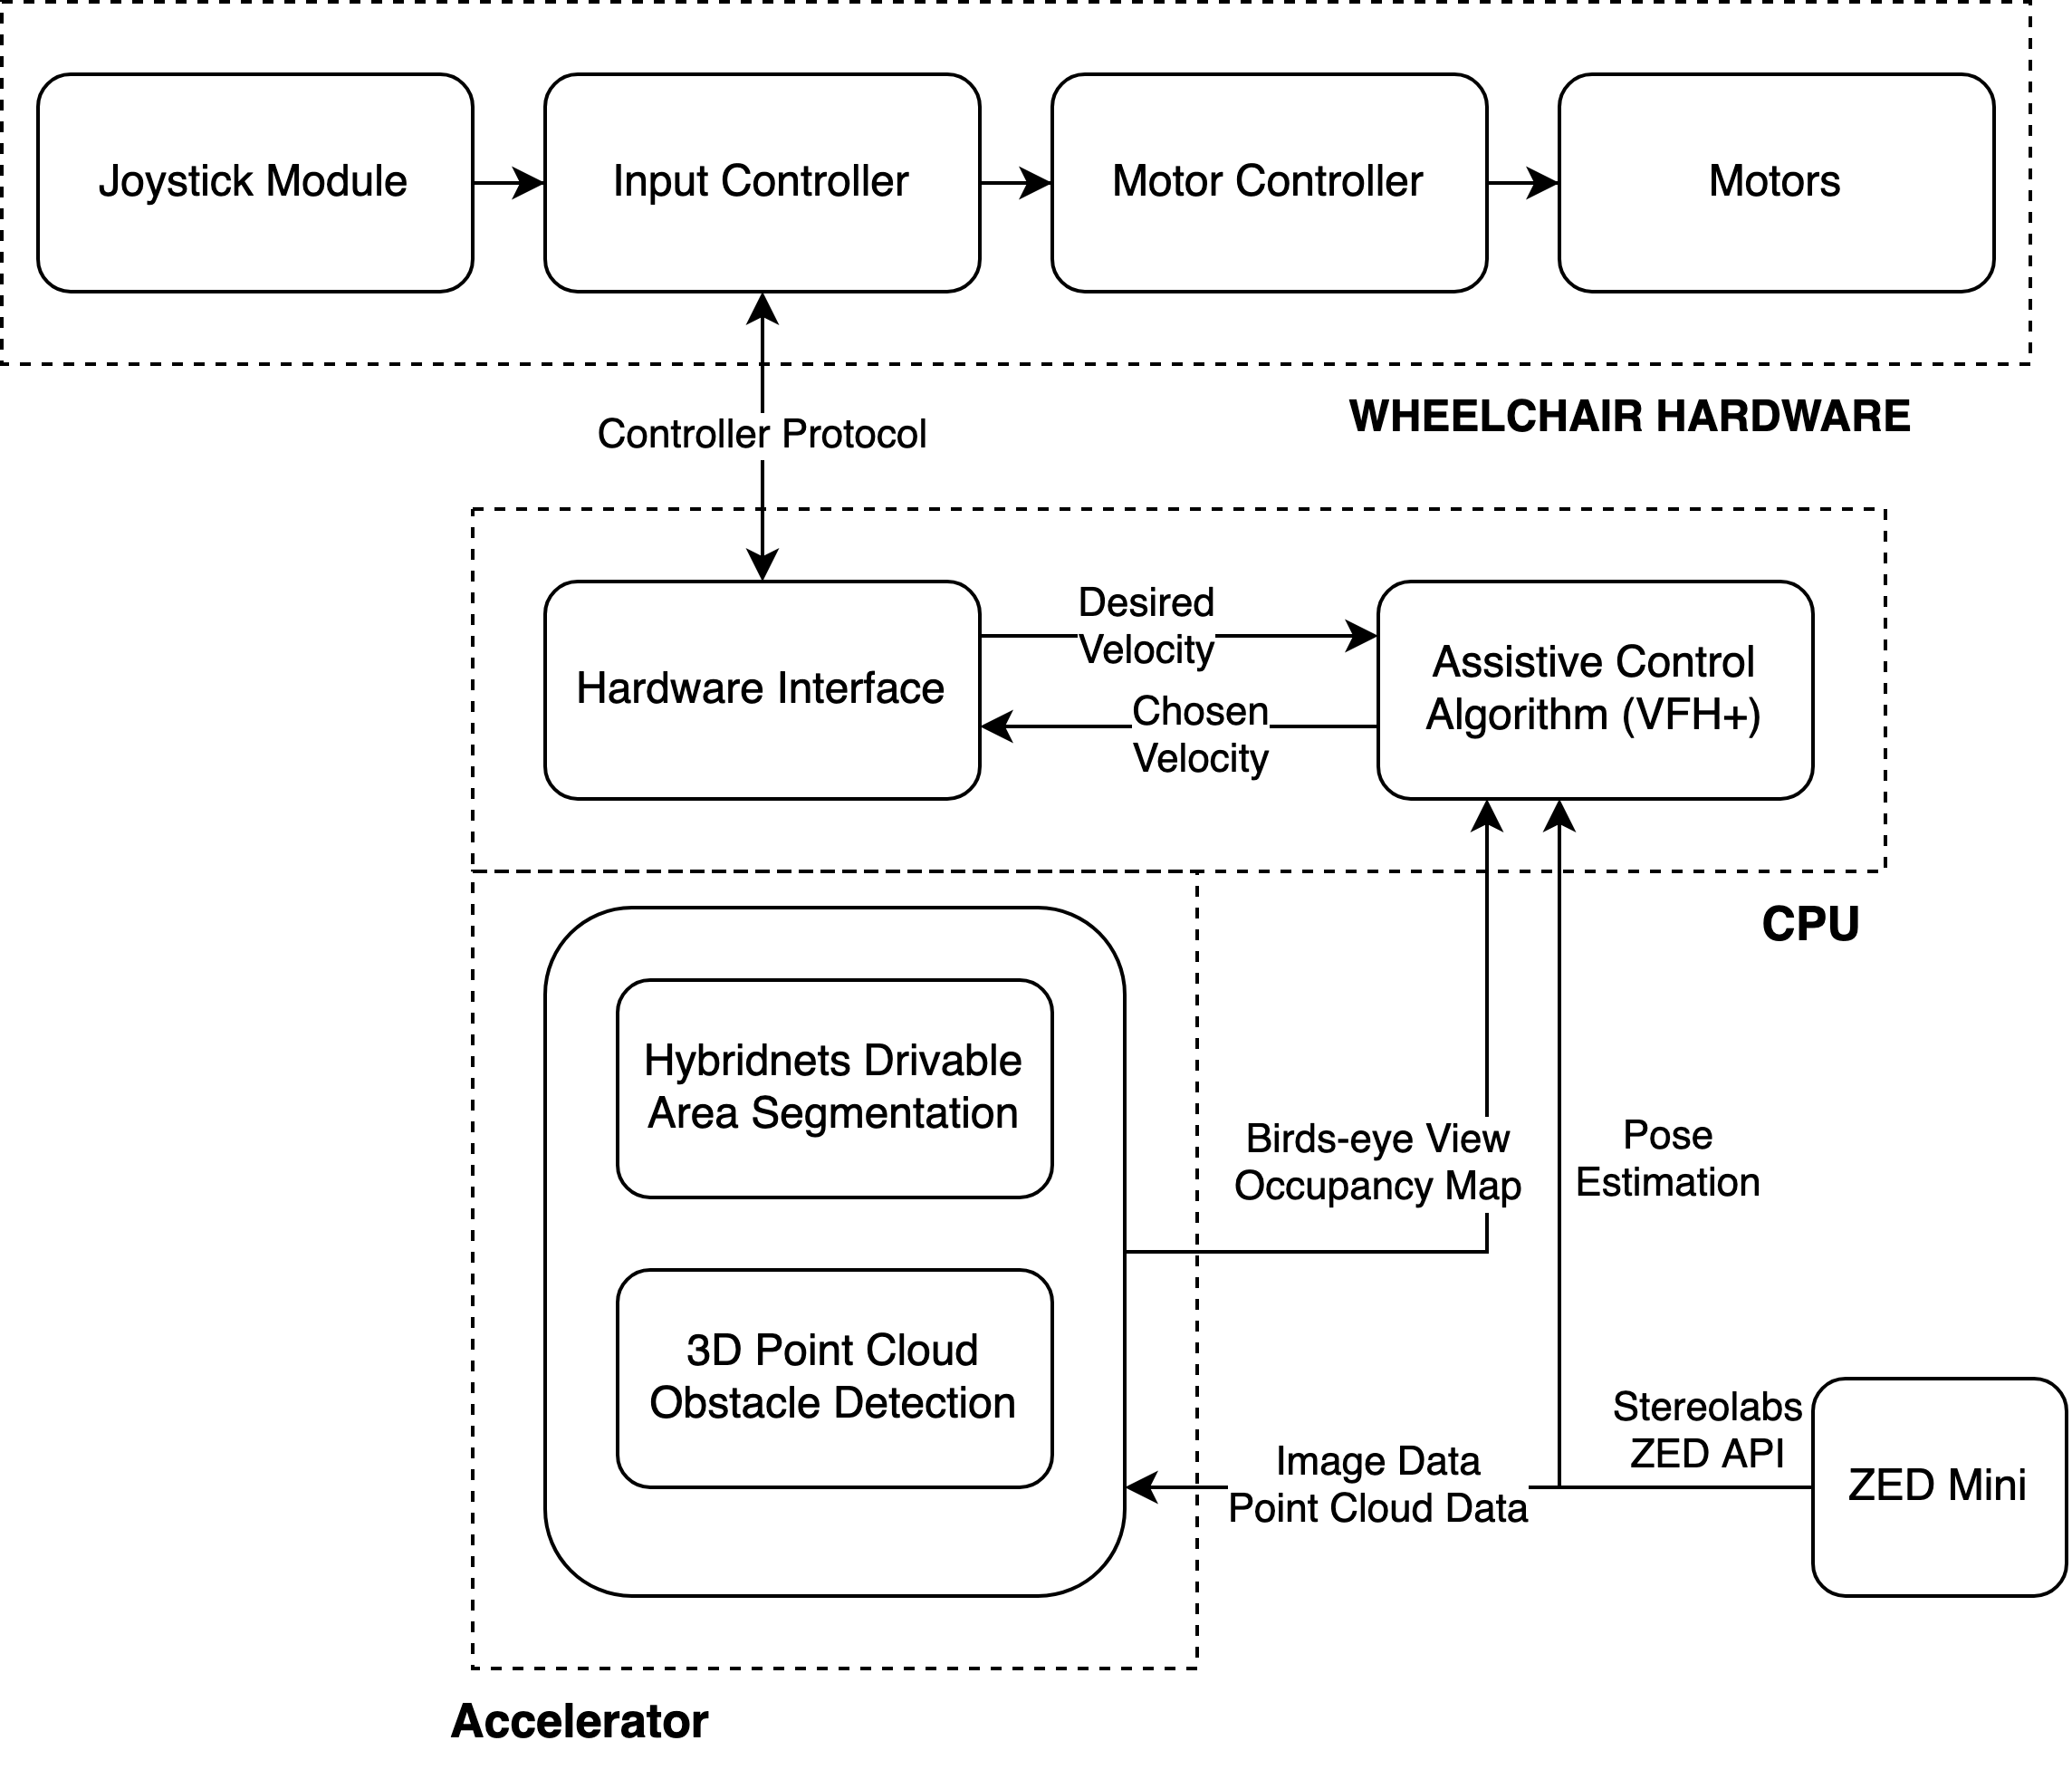
\includegraphics[width=0.8\linewidth]{images/block_diagram.png}
    \caption{Block diagram of software system and interaction with hardware components}
    \label{fig:block_diagram}
\end{figure}\clearpage

\subsection{Software}
The software system involves several scene recognition algorithms to update an internal
map of the surrounding area, keeping track of suitable driving paths and static obstacles
such as walls and stairs. Once this map is created, an algorithm blends the
user's input with this information to determine a safe path forward.
Appendix B contains a link to the source code. A block diagram of the software system
and how it interacts with the hardware is shown in \cref{fig:block_diagram}.

\subsubsection{Evaluation of ML models on preliminary dataset}
The preliminary video-only driving dataset was used to evaluate
several machine learning models before the ZED Mini had been ordered.
Object detection models such as YOLOv5 \cite{ultralyticsYOLOv5} and image segmentation models such as
DeepLabv3 \cite{chenRethinkingAtrousConvolution2017} were evaluated for speed, accuracy, and efficacy.
Hybridnets \cite{vuHybridNetsEndtoEndPerception2022}, a machine learning model which
performs drivable area segmentation and object detection on the same backbone, was also evaluated on
this dataset.

To evaluate these models, a video encoder and decoder needed to be created
to feed image frames into the model. This was implemented using a python generator
so that frames in the video could be iterated over within a for loop and only decoded
when required. OpenCV \cite{bradskiOpenCVLibrary2000} was the underlying library used
to decode each video frame into a BGR pixel array.
Some scene processing algorithms do not run in real-time due to hardware limitations or performance issues.
When this occurs, some frames must be dropped during model evaluation to keep the scene model up to date and minimise latency.
The number of frames to drop can be calculated using \cref{eq:frames_to_drop},
where $t_{frame}$ is the time taken to process the previous frame.
A frame is dropped by simply discarding it once decoded.

\begin{equation}
n_{drop} = \ceil{fps\times t_{frame}} - 1
\label{eq:frames_to_drop}
\end{equation}

To avoid training each model from scratch, a pre-trained model is loaded from PyTorch Hub.
The DeepLabv3 and YOLOv5 models were both trained on the MS COCO \cite{linMicrosoftCOCOCommon2014} dataset,
while the Hybridnets model was trained on the Berkeley DeepDrive dataset \cite{yuBDD100KDiverseDriving2018} (BDD100K).

%First, the ZED SDK is used to communicate with the ZED Mini camera and retrieve image data,
%point cloud data, and depth map data. Next, several scene recognition algorithms
%identify drivable areas and environmental obstacles. A block diagram of the software system
%and how it interacts with the hardware is shown in \cref{fig:block_diagram}.

As mentioned in the literature review, some machine learning algorithms can accept
different image classifiers as a model backbone.
MobileNetV3 \cite{howardSearchingMobileNetV32019} was used as a backbone for DeepLabv3 due to its fast performance.
YOLOv5 has 5 model backbones to choose between (nano, small, medium, large, extra-large),
with smaller models sacrificing accuracy for speed. Due to the low latency requirements
of a fast-moving wheelchair, YOLOv5 was evaluated using the small model size (known as YOLOv5s).
Machine learning was done using PyTorch \cite{paszkePyTorchImperativeStyle2019}, due to good compatibility
with existing machine learning models.

\subsubsection{Hybridnets drivable area segmentation}
To test the performance of the Hybridnets drivable area segmentation model,
the model was evaluated on the BDD100K and Cityscapes \cite{cordtsCityscapesDatasetSemantic2016}
datasets. The model was also retrained using the Cityscapes dataset
to improve its performance on non-uniform surfaces such as paved brick.

Machine learning was done within the Google Colaboratory environment,
and a Colab Pro subscription was purchased to enable access to
a faster Nvidia V100 GPU (with 16GB memory \cite{nvidiaNvidiaTeslaV1002018}).
Datasets were uploaded onto Google Drive so that they could be mounted onto Colab
and unzipped into the allocated machine's storage. Pytorch was used to train
the model, with \texttt{torchvision.datasets.Cityscapes} used to load the Cityscapes
dataset. To load the BDD100K dataset, a data loader within the Hybridnets source code
was used.

% could be added back for kerb detection
The Hybridnets model contains an image classification backbone, an object
detection head, and a segmentation head. The final layer of the segmentation head
was modified so that it would output only drivable area predictions, rather
than both lane predictions and drivable area predictions.
The weights for the backbone and detection head were `frozen', which means
they were not changed during training. This is standard practice when training
large models such as these, and reduces the time taken to train the model.

The mIoU (mean intersection over union) metric was used to evaluate the
performance of the model. \Cref{eq:miou} can be used to calculate the mIoU
which relies on the true positive, false positive, and false negative
pixel counts in the segmented image.

\begin{equation}
mIoU = \frac{1}{N} \sum_{i=1}^{N} \frac{tp_i}{tp_i + fp_i + fn_i}
\label{eq:miou}
\end{equation}

The Cityscapes dataset was selected to improve the model's performance on non-uniform
surfaces such as paved brick. This dataset includes sidewalks as well as roads;
this was hypothesised to provide a wider variety of surfaces during training.
Both sidewalks and roads were classified as drivable areas during evaluation
and training.

Recall (true positive rate, $\frac{tp}{tp + fn}$) was used as a metric to quantify the model's
performance on sidewalks and roads separately.
The AdamW optimizer \cite{kingmaAdamMethodStochastic2014}\cite{loshchilovDecoupledWeightDecay2017} was
used during training, with the model weights and other metrics saved to Google Drive
each epoch. The model was trained for 20 epochs in total.

%% Training methodology will likely take a while to write.
%This model was used to identify
%which areas were suitable for the wheelchair user to drive on,
%and as a proof of concept for a shared-backbone model architecture.

\subsubsection{Birds-eye view occupancy map}
\label{sec:birds_eye_view_occupancy_map}
%The 3D point cloud data was used to identify the corresponding location of a drivable segmented pixel in 3D space.
%This data was used to build a birds-eye view occupancy map of the local area, extending \SI{15}{\metre}
%in front of the wheelchair and \SI{5}{\metre} on either side.
%Large numerical computations were done using Numpy due to efficiency and ease of use.

The output of the Hybridnets drivable area segmentation model is a
segmentation mask, an array that indicates which pixels are drivable
and which are not.
This output must be transformed into a 2D birds-eye view occupancy map,
which indicates the drivable area around the wheelchair. The occupancy
map extends \SI{15}{\metre} in front of the wheelchair and \SI{5}{\metre} on either side.
This occupancy map is a simplified representation of the surrounding world
and is used as an input to the wheelchair control algorithms.

The ZED Mini 3D point cloud data was used
to transform the segmentation mask into an occupancy map.
The ZED SDK uses the pinhole camera model, as seen in \cref{fig:pinhole_camera_model},
to describe the relationship between pixels on the image plane
and the coordinates of corresponding objects.
The point cloud data is represented as an array the same size as
the original image, with each pixel containing XYZ data about the location of that object
in 3D space.
% add representation diagram
\begin{figure}[b]
    \centering
    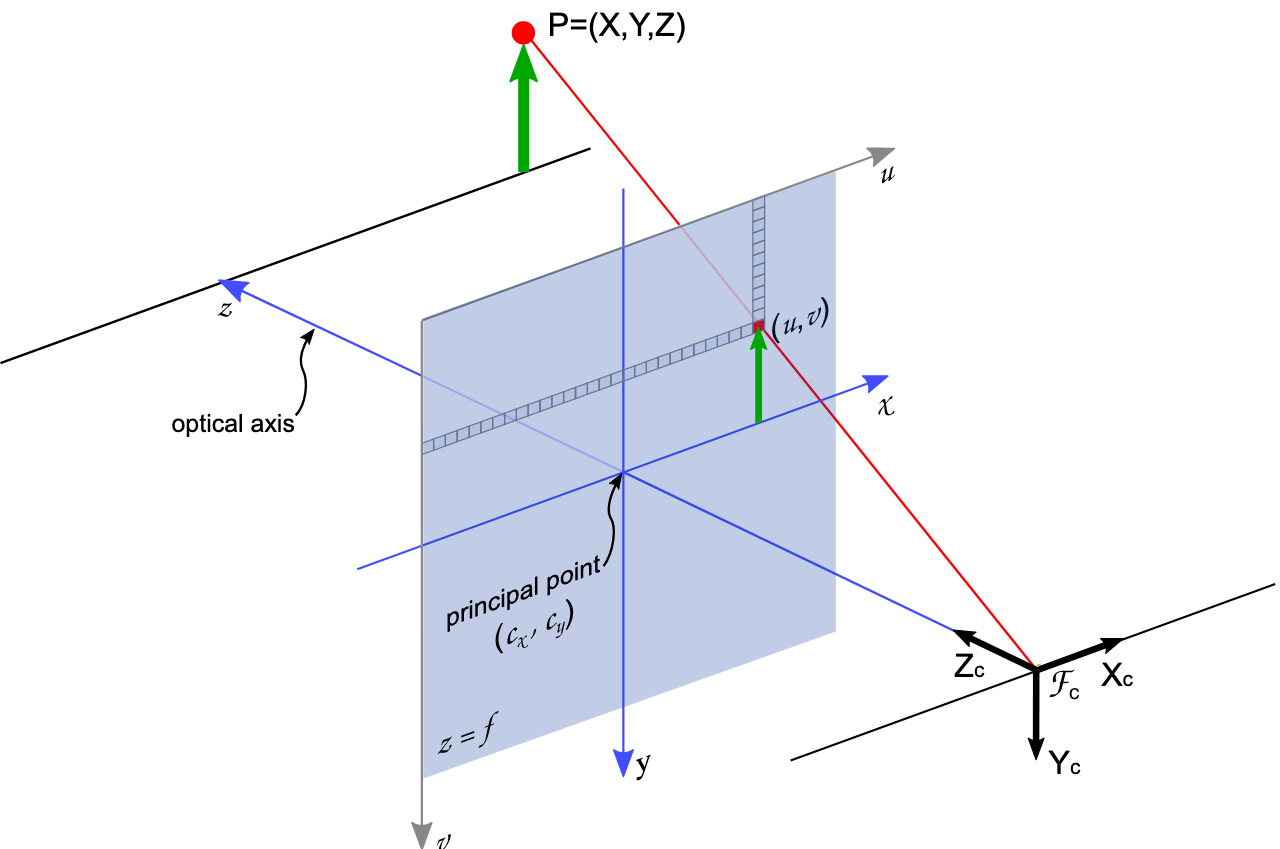
\includegraphics[width=0.8\linewidth]{images/pinhole_camera_model.png}
    \caption{Pinhole camera model. Reproduced from Nvidia \cite{nvidiaVisionProgrammingInterface}}
    \label{fig:pinhole_camera_model}
\end{figure}

To obtain the occupancy map, the point cloud is first filtered using the segmentation mask so that
non-drivable points are removed. The ZED SDK is unable to resolve the depth of some pixels
and instead represents their location as \texttt{nan}; these points are also removed.
Next, the array is simplified by removing non-essential information such as colour and altitude
data. What remains is an array of XZ points that represent drivable areas
identified by the segmentation algorithm. These XZ points are referenced
using a right-handed y-up coordinate frame, with the origin at the left lens of the ZED Mini;
see \cref{fig:zed_mini_coordinate_frame}.
\begin{figure}[b]
    \centering
    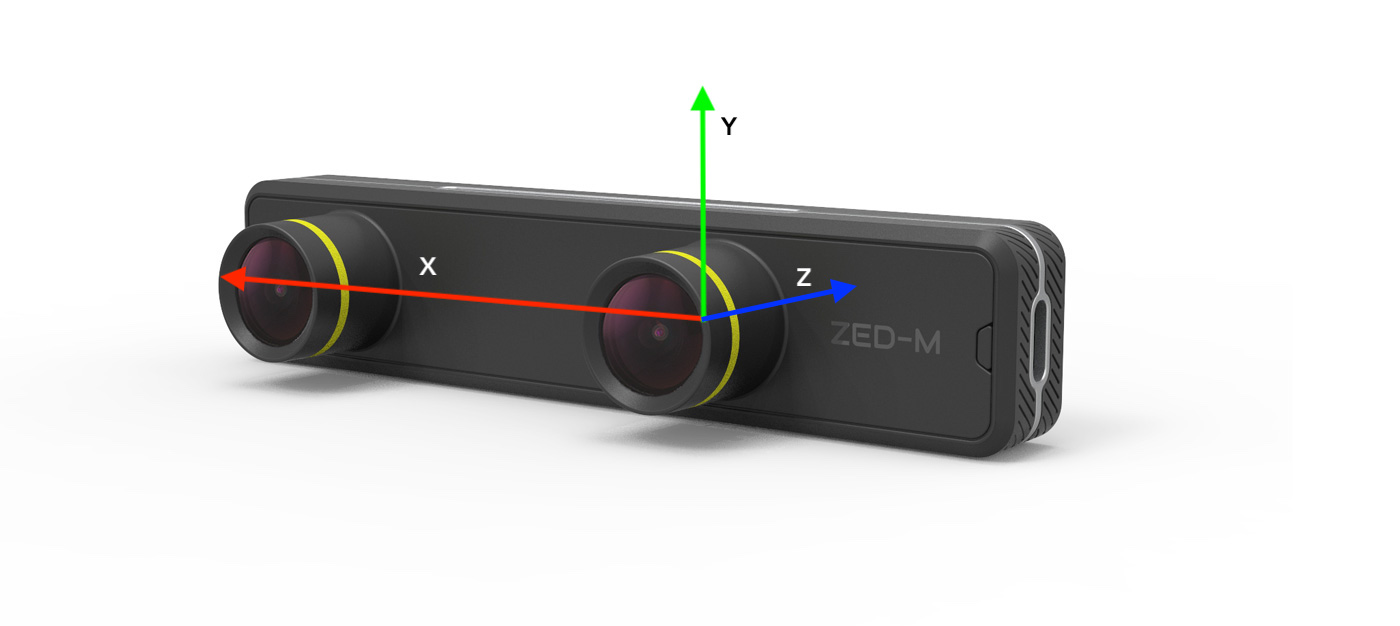
\includegraphics[width=0.8\linewidth]{images/zed_mini_coordinate_frame.jpg}
    \caption{ZED Mini coordinate frame (right-handed y-up)}
    \label{fig:zed_mini_coordinate_frame}
\end{figure}
% Add frame of reference

These points must be scaled to place them on the occupancy map. This occupancy map
extends \SI{15}{\metre} in front of the wheelchair and \SI{5}{\metre} on either side,
with each cell of the grid corresponding to a $\SI{25}{\milli\metre}\times \SI{25}{\milli\metre}$ area.
\Cref{eq:occupancy_scaling} was used to scale these points. Note that $p_x$ and $p_z$ are
represented in metres.

\begin{equation}
\begin{split}
i_x = min\left(max\left(\frac{p_x + 5.0}{0.025}, 1\right), \frac{10.0}{0.025}\right) - 1\\
i_y = min\left(max\left(\frac{p_z + 15.0}{0.025}, 1\right), \frac{15.0}{0.025}\right) - 1
\end{split}
\label{eq:occupancy_scaling}
\end{equation}

An issue with the occupancy map at this stage is that it is rather sparse
due to the one-to-one mapping between segmented pixels and grid cells.
Morphological image processing techniques were used to improve the density of the occupancy map.
The OpenCV \cite{bradskiOpenCVLibrary2000} implementation of morphological dilation was used to
join the space between drivable pixels, to create a continuous driving surface in the occupancy map
rather than many separate pixels. A $10\times 10$ kernel was used to perform this dilation.

\pagebreak
\subsubsection{3D point cloud obstacle detection}
\label{sec:point_cloud_obstacle_detection}

Another method that was tested to identify environmental obstacles and drivable areas
was the direct processing of the 3D point cloud data, which removes any use of RGB image data.
One approach that was tested was the inbuilt ZED SDK function \texttt{find\_floor\_plane}.
This function takes the current floor height and camera orientation as arguments
and uses them to identify the floor plane. The \texttt{find\_floor\_plane} function
returns a 3D polygon of the floor plane boundary, which was projected onto the 2D XZ plane
and displayed using the python Pillow library.
% add find_floor_plane results

Another approach that was tested was a custom algorithm that processes the 3D point cloud data
to identify the drivable area.
The inequality in \cref{eq:flat_filter} was initially used to filter the points
which were identified as drivable,
using a measured camera height $y_{camera} = \SI{740}{\milli\metre}$
and an initial error parameter $y_{error} = \SI{150}{\milli\metre}$.
\Cref{eq:flat_filter} only retains 3D points within a certain error margin of the floor plane.

\begin{equation}
-y_{error} \leq p_y + y_{camera} \leq y_{error}
\label{eq:flat_filter}
\end{equation}

An issue with this equation is that it does not take camera tilt into account.
Additionally, a wheelchair ramp may not be recognised as drivable, as the gradient of a ramp
may cause sections of the ramp to fall outside the $y_{error}$ margin.
Australian Standard 1428.1:2021 \cite{standardsaustralia14282021Design2021} specifies that
the maximum gradient of a wheelchair ramp should not be greater than 1:14 (section 7.3a).

To rectify these issues, \cref{eq:tilt_filter} was also tested to identify the drivable area.
This approach takes sensor tilt and wheelchair ramps into account,
assuming that any ramps will be encountered face-on (along the z-axis) and that
sensor tilt remains constant. Note that in our coordinate system,
$p_z$ is negative in front of the wheelchair.

\begin{equation}
\begin{split}
p_h = p_y - &p_z\tan\theta_{tilt} + y_{camera}\\
p_z\times\frac{1}{14} - y_{error} &\leq p_h \leq -p_z\times\frac{1}{14} + y_{error}
\end{split}
\label{eq:tilt_filter}
\end{equation}

Direct processing of the 3D point cloud data was also tested to detect static obstacles,
such as stairs and walls. A basic implementation was tested using the existing sensor
tilt compensation in \cref{eq:tilt_filter}. \Cref{eq:obstacle_filter} shows the point filtering
criteria for obstacles between \SI{0.5}{\metre} and \SI{2.0}{\metre} tall.

\begin{equation}
0.5 \leq p_h \leq 2.0
\label{eq:obstacle_filter}
\end{equation}

Once the 3D points for drivable areas and environmental obstacles have been identified,
they must be placed on the birds-eye view occupancy map. The approach used to do this
is identical to the approach outlined in \cref{sec:birds_eye_view_occupancy_map};
each point is scaled to fit on the map and morphology is used to improve the density
of this map.

\subsubsection{Assistive control algorithm}
The VFH+ (vector field histogram) algorithm \cite{ulrichVFHReliableObstacle1998} was used to blend
the user's desired direction with the occupancy map to determine a safe target direction.
One limitation of the VFH+ algorithm is that it only adjusts the direction of the wheelchair
and not the wheelchairs speed; as such, this algorithm was implemented as a
proof of concept rather than a complete assistive control algorithm.
The occupancy map generated by the 3D obstacle detection algorithm (detailed in \cref{sec:point_cloud_obstacle_detection})
was used as the input into the VFH+ algorithm.

This algorithm was implemented in MATLAB using the Navigation toolbox and encapsulated into a MATLAB function.
The `MATLAB Engine' Python API was used to call the assistive control algorithm from within Python code.
Full implementation of a control algorithm would require the ability to log joystick commands during
data collection, and to intercept joystick commands from the user. As the input controller had not
been implemented at this time, the user's desired direction was assumed to be the current direction
of the wheelchair.

As the VFH+ control algorithm had already been implemented within the Navigation toolbox,
the MATLAB implementation was relatively simple. \Cref{eq:pose_adjustment} was used to adjust
the pose from the RGB-D camera to the centre of the wheelchair.

\begin{equation}
\begin{split}
p_{wheelchair,x} &= p_{camera,x} - \frac{w_{wheelchair}}{2}\\
p_{wheelchair,y} &= p_{camera,y} + \mathrm{offset_{sensor}} - \frac{l_{wheelchair}}{2}
\end{split}
\label{eq:pose_adjustment}
\end{equation}

\subsubsection{Pose estimation}
Pose estimation allows the smart wheelchair to update its position within the surrounding world.
The ZED Sensors API and ZED Positional Tracking API were tested to estimate the pose of the wheelchair.
These APIs were tested as a proof of concept for pose estimation and were not directly used
for assistive control.

%This is important for mapping and control, as it requires 
%The wheelchair can be modelled as a 2 wheeled differential drive robot, which means that the
%instantaneous velocity of the wheelchair
\pagebreak
The Sensors API performs pose estimation using 6 DOF IMU sensor fusion and can also output raw accelerometer
and gyroscope data. Although the IMU has a sampling rate of \SI{800}{\hertz}, this sensor information
is only saved to the SVO file at the camera frame rate of \SI{30}{\hertz}.

The Positional Tracking API combines sensor data with image data to track the camera's movement.
The camera's movement can be specified using two coordinate frames: CAMERA and WORLD.
The WORLD frame outputs the position of the camera relative to the point where the ZED Mini started
motion tracking ($P_i$), while the CAMERA frame outputs the difference between the current camera position and
the camera position in the previous image ($\Delta P$).

Another method to calculate $\Delta P$ would be to store the previous camera pose
and use \cref{eq:pose_estimation} to calculate the difference between consecutive poses.
% add 2 wheeled differential kinematics here

\begin{equation}
\begin{split}
P_i \Delta P &= P_{i+1}\\
\Delta P &= P_i^{-1} P_{i+1}
\end{split}
\label{eq:pose_estimation}
\end{equation}

An advantage of this approach over using the CAMERA reference frame is that if a frame
is skipped due to performance or latency issues, no movement data is lost.
Performance should not be a concern, as the inversion of a pose matrix can be done
very efficiently.

% add 2 wheeled differential drive robot diagram

%The 3D point cloud data was used to identify the corresponding location of a drivable segmented pixel in 3D space.
%This data was used to build a birds-eye view occupancy map of the local area, extending \SI{15}{\metre}
%in front of the wheelchair and \SI{5}{\metre} on either side.
%Large numerical computations were done using Numpy due to efficiency and ease of use.

%Morphological image processing techniques were used to improve the density of the occupancy map.
%The OpenCV \cite{bradskiOpenCVLibrary2000} implementation of morphological dilation was used to
%join the space between drivable pixels, to create a continuous driving surface in the occupancy map
%rather than many separate pixels.

%Manual processing of the 3D point cloud data was also tested to identify the floor plane and drivable area.
%This approach was compared with the inbuilt \texttt{find\_floor\_plane} ZED API function.
%Environmental obstacles between the heights of \SI{0.5}{\metre} and \SI{2.0}{\metre} were
%detected using the 3D point cloud data and added to the occupancy map.

% MATLAB camera -> center of wheelchair transform?
%The VFH+ (vector field histogram) algorithm \cite{ulrichVFHReliableObstacle1998} was used to blend
%the user's desired direction with the occupancy map to determine a safe target direction.
%This algorithm was implemented in MATLAB using the Navigation toolbox. The `MATLAB Engine' API
%was used to transfer data between Python and MATLAB code.
%As the input controller had not been implemented yet, joystick commands could not be logged; instead,
%the user's desired direction was assumed to be the current direction of the wheelchair.

%The ZED Sensors API and ZED Positional Tracking API were tested to track the movement of the wheelchair.
%The Sensors API performs pose estimation using 6 DOF IMU sensor fusion and can also output raw accelerometer
%and gyroscope data. The Positional Tracking API combines sensor data with image data to track the camera's movement.
